\documentclass[9pt]{pnas-new}
% Use the lineno option to display guide line numbers if required.
% Note that the use of elements such as single-column equations
% may affect the guide line number alignment. 

%\RequirePackage[english,slovene]{babel} % when writing in slovene
\RequirePackage[slovene,english]{babel} % when writing in english
\DeclareUnicodeCharacter{202F}{ }
\templatetype{pnasresearcharticle} % Choose template 
% {pnasresearcharticle} = Template for a two-column research article
% {pnasmathematics} = Template for a one-column mathematics article
% {pnasinvited} = Template for a PNAS invited submission
\usepackage{graphicx}
\usepackage{subcaption}
\usepackage{adjustbox}
\selectlanguage{english}
%\etal{in sod.} % comment out when writing in english
%\renewcommand{\Authands}{ in } % comment out when writing in english
%\renewcommand{\Authand}{ in } % comment out when writing in english

\newcommand{\set}[1]{\ensuremath{\mathbf{#1}}}
\renewcommand{\vec}[1]{\ensuremath{\mathbf{#1}}}
\newcommand{\uvec}[1]{\ensuremath{\hat{\vec{#1}}}}
\newcommand{\const}[1]{{\ensuremath{\kappa_\mathrm{#1}}}} 

\newcommand{\num}[1]{#1}

\graphicspath{{./fig/}}

\title{Swarming behaviour in predator-prey model}

% Use letters for affiliations, numbers to show equal authorship (if applicable) and to indicate the corresponding author
\author{Ariana Kržan}
\author{Tina Brdnik}
\author{Vito Levstik}

\affil{Collective behaviour course research seminar report} 

% Please give the surname of the lead author for the running footer
%\leadauthor{Lead author last name} 

\selectlanguage{english}

% Please add here a significance statement to explain the relevance of your work
\significancestatement{Here goes significance statement.}{Simulation | swarming behaviour | predator | prey}

\selectlanguage{english}

% Please include corresponding author, author contribution and author declaration information
%\authorcontributions{Please provide details of author contributions here.}
%\authordeclaration{Please declare any conflict of interest here.}
%\equalauthors{\textsuperscript{1}A.O.(Author One) and A.T. (Author Two) contributed equally to this work (remove if not applicable).}
%\correspondingauthor{\textsuperscript{2}To whom correspondence should be addressed. E-mail: author.two\@email.com}

% Keywords are not mandatory, but authors are strongly encouraged to provide them. If provided, please include two to five keywords, separated by the pipe symbol, e.g:
\keywords{Simulation | swarming behaviour | predator | prey} 

\begin{abstract}
    Collective animal behaviour, especially swarming in predator-prey dynamics, offers insights into survival strategies 
    that emerge under evolutionary pressures. This report outlines the initial objectives and foundational concepts for simulating 
    predator-prey. Inspired by previous work, we examined how survival pressures can drive emergent group behaviours
    in prey through reinforcement learning. 
    Our primary objective was to recreate a reinforcement learning-based model where predator-prey interactions lead to swarming 
    and evasion behaviours. Unfortunately, we have not been able to observe any swarming behaviour. We suspect that the rewards used in the model lead
	to suboptimal results. With different learning parameters we might be able to achieve desired results, but so far we have not been able to do so.
	The model was then extended to include environmental obstacles and an additional species, 
    to provide framework for future work on interspecies interactions and new survival strategies.
\end{abstract}

\dates{\textbf{\today}}
\program{BMA-RI}
\vol{2024/25}
\no{Group G} % group ID
%\fraca{FRIteza/201516.130}


\begin{document}

% Optional adjustment to line up main text (after abstract) of first page with line numbers, when using both lineno and twocolumn options.
% You should only change this length when you've finalised the article contents.
\verticaladjustment{-2pt}

\maketitle
\thispagestyle{firststyle}
\ifthenelse{\boolean{shortarticle}}{\ifthenelse{\boolean{singlecolumn}}{\abscontentformatted}{\abscontent}}{}

% If your first paragraph (i.e. with the \dropcap) contains a list environment (quote, quotation, theorem, definition, enumerate, itemize...), the line after the list may have some extra indentation. If this is the case, add \parshape=0 to the end of the list environment.
\dropcap{T}he sudden emergence of swarming behaviours in animals is one of the most striking examples of collective animal behaviour. 
These behaviours have been extensively studied for their implications for the evolution of cooperation, 
social cognition and predator–prey dynamics \cite{olson2013predator}. Swarming, which appears in many different species like starlings, 
herrings, and locusts, has been linked to several benefits including enhanced foraging efficiency, improved mating success, and distributed problem-solving abilities. 
Furthermore, they are hypothesized to help with improving group vigilance, reducing the chance of being encountered by predators, 
diluting an individual's risk of being attacked, enabling an active defence against predators and reducing predator attack efficiency by confusing the predator \cite{li2023predator}.

In this project we took the inspiration from the work of Li et al. (2023) \cite{li2023predator} to explore how simple survival pressures can drive the emergence of swarming behaviour. 
The first goal was to create a realistic simulation where both prey and predators learn to adapt through reinforcement learning based on their drive to survive.
Unfortunately, we have not yet been able to recreate the same results as in \cite{li2023predator} or at least observe any swarming behaviour.

Nevertheless, we then extend our work by providing framework for the introduction of new environmental obstacles and new species with the desire to observe how interspecies interactions lead to new survival strategies.

\section*{Methods}

Our proposed methodology aimed to simulate swarming behaviours in a predator-prey environment using reinforcement learning (RL). 
We defined and tested a RL-based model where agents, such as prey and predators interacted within a two-dimensional space. The goal was to observe collective behaviours like swarming, evasion, and strategic movement.

We implemented our own environment setup, which we wanted to compare with the model from Li et al. (2023) \cite{li2023predator}.

\subsection{Environment Setup}
The simulation took place in a 2D environment with open space, meaning that agents reappeared on the opposite side when they crossed the boundary.
Such setup with periodic boundaries serves as an approximation of an infinite space, where agents are allowed to move freely without encountering physical borders. 
Later on, we introduced a new species to the environment and placed random obstacles, which simulated more realistic and complex space that challenged the agents to adapt their movement and coordination. 

\subsection{Agent Dynamics}
Agents in our simulations were subject to both active and passive forces.

\textbf{Active forces} are self-generated by agents to drive their movement. These forces consist of two components:
\begin{itemize}
	\item \textbf{Forward Propulsion}: Drives the agent in the direction of its heading. This force is represented as \( a_F \).
	\item \textbf{Rotational Force}: Allows the agent to rotate its heading within a threshold value. This force is denoted as \( a_R \), where \( a_R \) controls the angular velocity.
\end{itemize}

\textbf{Passive forces} act on agents due to interactions with the environment and other agents. These include:
\begin{itemize}
	\item \textbf{Dragging Force}: Acts opposite to the agent's velocity, simulating frictional effects. It is proportional to the magnitude of the velocity \( \vec{v} \).
	\item \textbf{Elastic Forces Between Agents}: When agents are in contact, elastic forces prevent overlap and simulate collision dynamics. These forces follow Hooke's law and are represented as \( \vec{f}_a \).
\end{itemize}

The RL framework aimed to optimize the agents' use of active forces \( a_F \) and \( a_R \) to maximize their survival behaviors.

\subsection{Agent Types and Behaviour}
\begin{itemize}
    \item \textbf{Prey}: Prey aims to survive by avoiding predators and moving as a group.
    \item \textbf{Predators}: Predators are designed to pursue and catch prey.
    \item \textbf{Super Predators}: We introduced a third type of agent called super predators. The aim of super predators is to catch predators, while not caring about the prey. This would simulate a real world food chain, where predators would have to choose between catching prey or avoiding super predators.
\end{itemize}

\subsection{Reinforcement Learning Framework} At first we wanted to use the Multi-Agent Deep Deterministic Policy Gradient (MADDPG) algorithm, but we had a hard time writing it from scratch. Hence, we later decided to use Proximal Policy Optimization (PPO) algorithm.

We followed the same reward structure as in Li et al. (2023) \cite{li2023predator}, where the reward for prey is set to $-1$ if it is caught by a predator and the predator is awarded $+1$ if it catches a prey. As in the original article we also added small penalty of $-0.01|a_F|-0.1|a_R|$ which mimics the cost of movement.
When adding super predators, we followed the same reward structure for the interaction between predators and super predators.

Agents were trained through episodic simulations, allowing them to learn and adapt from each episode's interactions. We varied parameters to try and get the best results, but so far we have not been successful.

\subsection*{Proposed Methodology for Verification}

To verify the behavior of our model, we adopted the methodology described in Li et al. (2023) \cite{li2023predator}, utilizing two key metrics: the Degree of Alignment (DoA) and the Degree of Separation (DoS).

\begin{itemize}
    \item \textbf{Degree of Sparsity (DoS):} This metric measures the spatial aggregation of agents, capturing how densely the agents cluster together. It is defined as:
    \[
    \text{DoS} = \frac{1}{TND} \sum_{t=1}^T \sum_{j=1}^N \| \mathbf{x}_j(t) - \mathbf{x}_k(t) \|
    \]
    where: \( \mathbf{x}_j(t) \) is the position of the \(j\)-th agent at time step \(t\), \( \mathbf{x}_k(t) \) is the position of the nearest neighbor \(k = \arg\min_k \| \mathbf{x}_j(t) - \mathbf{x}_k(t) \| \), \(T\) is the episode length, \(N\) is the total number of agents, and \(D\) is the maximum possible distance between two agents in the environment.
    
    A smaller DoS value indicates denser clustering, while a value of 0 represents all agents aggregating at a single point.

    \item \textbf{Degree of Alignment (DoA):} This metric quantifies the alignment of the agents' headings, assessing how consistently agents move in the same direction. It is defined as:
    \[
    \text{DoA} = \frac{1}{2TN} \sum_{t=1}^T \sum_{j=1}^N \| \mathbf{h}_j(t) + \mathbf{h}_k(t) \|
    \]
    where: \( \mathbf{h}_j(t) \) is the heading of the \(j\)-th agent at time step \(t\), \( \mathbf{h}_k(t) \) is the heading of the nearest neighbor of agent \(j\) (the same nearest neighbor as in the DoS calculation), \(T\) is the episode length, and \(N\) is the total number of agents.
    
    Higher DoA values indicate stronger alignment in agent movement. It is important to note that the DoA measures local alignment between neighboring agents rather than the mean heading of the entire group, making it more suitable for detecting relative alignment within swarms.
\end{itemize}

\section*{Results}


In the initial phase of our project, we implemented a basic model where we created our environment with periodic borders and successfully populated it with agents which followed a reward system following the article. At this stage we only implemented active forces with fixed values. Our results looked promising.

Now we have improved the model by first adding passive forces. We also fine-tuned some parameters such as the agents' speed, size and passive forces. 
The passive forces include dragging forces, elastic forces between contacting agents, and elastic forces between agents and boundaries. 
Next we initiated active forces as random instead of fixed valued. That was crucial for our next step, since we were gonna build our reinforcment model based on them.

Lastly we added a RL component. The RL component was built to fine-tune the active forces $a_f$ and $a_f$ to enable the agents to move efficiently and maximize their results. 
However so far, after successfully training our model numerous times over 1000 episodes, the results were not great. Instead of the agents moving to maximize their reward, they end up moving in circles.

\begin{figure}[ht]
	\centering
	% Subfigure (a)
	\begin{subfigure}{0.30\textwidth}
		\centering
		\fbox{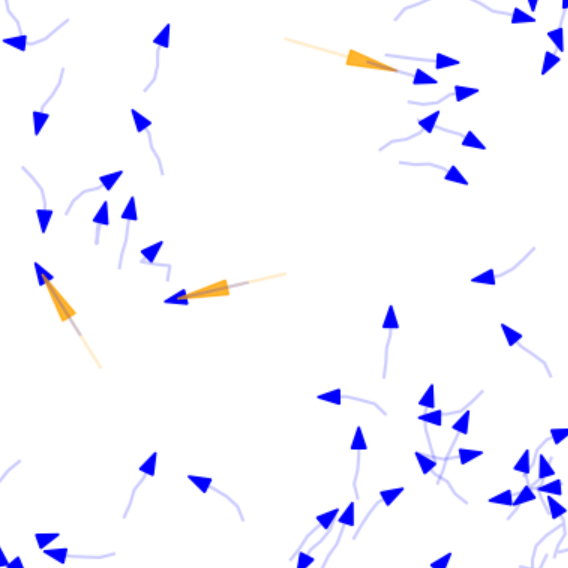
\includegraphics[width=\textwidth]{fig/reward.png}}
		\vspace{0.5em}
		\centering (a)
	\end{subfigure}
	\hfill
	% Subfigure (b)
	\begin{subfigure}{0.30\textwidth}
		\centering
		\fbox{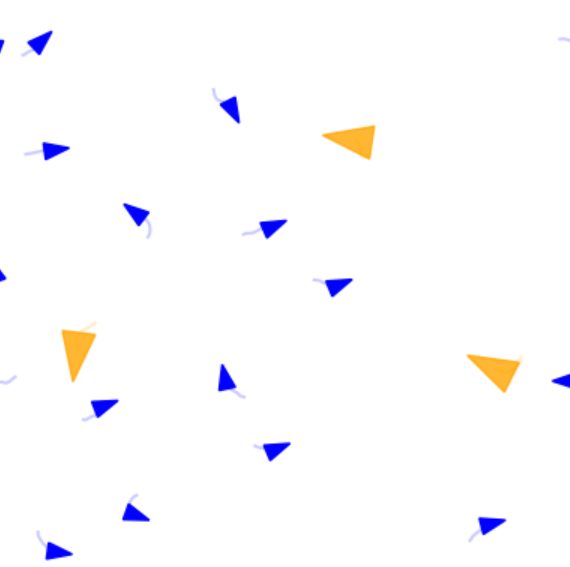
\includegraphics[width=\textwidth]{fig/basic2.png}}
		\vspace{0.5em}
		\centering (b)
	\end{subfigure}
	\hfill
	% Subfigure (c)
	\begin{subfigure}{0.30\textwidth}
		\centering
		\fbox{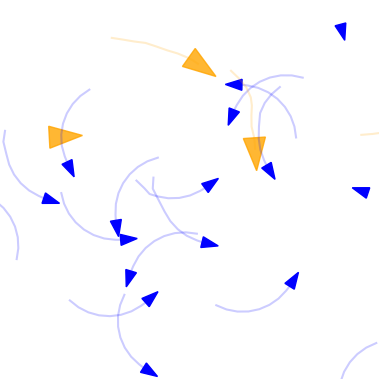
\includegraphics[width=\textwidth]{fig/withRL.png}}
		\vspace{0.5em}
		\centering (c)
	\end{subfigure}
	
	\caption{(a) Our model with no RL component, following the reward system and fixed active forces. (b) Our model with no RL component, with added fixed passive forces and random initialization of active forces (c) Our model with RL.}
	\label{fig:three_images}
\end{figure}

Recognizing these limitations, we decided to adopt the RL model from the Li et al. article \cite{li2023predator}.
Using their code, we were able to successfully run simulations of their model in our environment. 
This provided a functioning baseline for comparison and further experimentation.
Our results demonstrate significant progress in achieving swarming behaviors. 
Specifically, we achieved an impressive Degree of Separation (DoS) value of 0.12.
The prey agents were able to form tight clusters while escaping the predators.
However, the Degree of Alignment (DoA) results remained suboptimal, with values consistently staying at around 0.3.
This indicates that while agents were able to group closely, they struggled to align their velocities and directions cohesively. 
Even after consulting with the original authors we didn't get better results.

\begin{figure}[ht]
	\centering
	\begin{subfigure}{0.30\textwidth}
		\centering
		\fbox{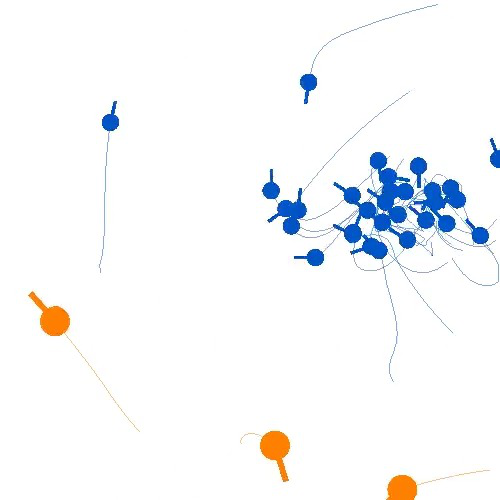
\includegraphics[width=\textwidth]{fig/swarming3.png}}
		\vspace{0.5em}
	\end{subfigure}
	\hfill
	\begin{subfigure}{0.30\textwidth}
		\centering
		\fbox{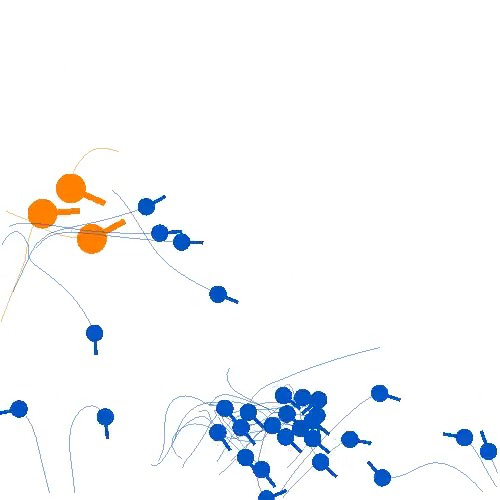
\includegraphics[width=\textwidth]{fig/swarming1.png}}
		\vspace{0.5em}
	\end{subfigure}
	\hfill
	\begin{subfigure}{0.30\textwidth}
		\centering
		\fbox{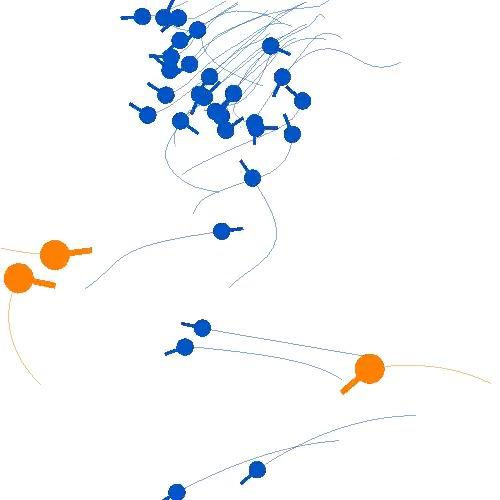
\includegraphics[width=\textwidth]{fig/swarming2.png}}
		\vspace{0.5em}
	\end{subfigure}
	
	\caption{Visualization of simulation results showing agent behavior. The prey demonstrate successful swarming behavior, as indicated by the tight clustering of prey, resulting in a low Degree of Separation. However, the also show poor alignment, leading to low DoA numbers.}
	\label{fig:three_images2}
\end{figure}


\section*{Discussion}
In this stage of the project, we successfully ran the code from the main article but encountered challenges with the agents' behavior. 
The DoA and DoS metrics remain highly variable, indicating that swarming behaviors have not yet emerged. 
These results suggest the need for further tuning of the reward structure and additional training.

Despite the setbacks, we are motivated to continue refining the model and addressing these issues. 
Our next steps are to improve the code to produce results similar to the article, introduce obstacles to the environment, and add a ecies, which we have yet to finalize.

\acknow{AK worked on models with and without RL component implementations and writing agent dynamics and results, TB worked on graphs, methods, results and discussion, VL worked on training and testing the original model.}
\showacknow % Display the acknowledgments section

% \pnasbreak splits and balances the columns before the references.
% If you see unexpected formatting errors, try commenting out this line
% as it can run into problems with floats and footnotes on the final page.
%\pnasbreak

\begin{multicols}{2}
	%\bibliographystyle{plain} % or any style you prefer, such as ieee, unsrt, etc.
	\bibliography{bib/bibliography} % This assumes your .bib file is located at ./bib/bibliography.bib
\end{multicols}


\end{document}
